\chapter{Design Specification}
\tableofcontents
\newpage
\section{Introduction}
\subsection{Purpose of Document}
The purpose of this document is to set out an initial design for the project 'Adapting Access Aber to android making use of native features'. It will encompass various design decisions and estimations of what the final system should look like on a code level. The final Design may differ but should lie around the boundaries set out here.
\subsection{Scope}
This Design Specification will split up the application into several components and describe any interaction within the application. Some components may essentially be stand alone except for the link to them however. This document may reference the requirements specification previously set out, it will likely reference the required functionality set out within the 'Functionality' section. For ease of use the following are the main areas of functionality required, these will be referenced by their key displayed here throughout the document. More details on each functional requirement can be found in the requirements specification.

\begin{itemize}
	\item FR1 - Route Finding - Guiding a User around campus
	\item FR2 - Route Plotting - Users must be able to plot their own routes.
	\item FR3 - Location Based Help - Provide details of possible help available.
	\item FR4 - Building Display - A display of related buildings
	\item FR5 - Multi Lingual Support - Welsh translation
\end{itemize}
 

\subsection{Objectives}
The objectives of this document are to - 
\begin{enumerate}
\item Describe the main components of the Access Aber Application (AA)\cite{aa}
\item Provide Details of interactions performed by the Application
\item To provide details about likely class interfaces
\item To provide diagrams of significant data structures and details of significant algorithms 
\end{enumerate}
\newpage
\section{Decomposition Description}
The decomposition description will provide details on the division of the modules which make up the application. It describes the structure of the system and the function of each significant module. This should give a good overview of the expected design in an abstract way. 
\subsection{Modules within the Application}
This section will describe how we expect the application to be split up for development. Due to the singular nature of most of the application, it is likely development will take place by feature rather than as a whole.

The application itself is expected to be split into 4 main modules which will be accessed through a central menu. 
\begin{enumerate}
\item A route finder for users to enter a start and destination and have a route displayed to them.
\item A help service which provides details on the closest possible person who may be able to provide help.
\item A display of buildings that the user can filter.
\item A Route plotter to help the maintainers plot routes while seeing them and the current route they're plotting. 
\item It is also possible a separate application will be developed to test the loading of route files created by the application.
\end{enumerate}
The following section will detail further design elements related to the expected modules.
\subsubsection{Route Finder}
The route finder is where the main source of issues is expected to come from, the representation of data and searching of that data is expected to pose problems and take a fair amount of time to perfect. However some steps have been taken already to research possible ways to solve this task. A searchable graph is required to avoid the issue seen in the initial web application of having too many saved routes. 

It is expected that a Breadth First Search (BFS)\cite{bfs} will be used, this is due to the guarantees it can provide us and past experience. Using BFS should mean we will provide the shortest path in terms of locations traversed, while this may not guarantee the definitive shortest path the layout of campus and the graph that is expected to be used means the least locations should always mean the least distance. While BFS can sometimes be heavy on memory use due to it storing every node on a specific 'level' it is not expected that the graph used will be overly large so issues relating to this should be mostly avoided. This also helps us combat the time issue. In a larger environment we would have significant problems and if this application is adapted in future this search may need to be swapped out for another.

Each Node will essentially be a traversable location, whether the location is a destination or not is another matter. With initial research it is obvious that the graph will have to abide by the road and walkway system within the Universities campus, so some locations may be junctions in walkways. Due to this each link between each Node should be represented as a set of Co Ordinates which we can then plot on the map provide through Google Play Services. 

It has already been decided that in an ideal solution no location will be hard coded and instead loaded in from files who follow a set format and as such can be made with the Route Plotting application to meet FR2. The source of these files is expected to be within the applications own assets, however research will be done on fetching the files from a server to see if it provides any significant benefits. Files retrieved from the internet would mean we did not need to push an update every time something changed, however it is unlikely campus will change significantly and updates should not be too common. Thus meaning local files is probably an acceptable solution especially considering the issues posed by poor signal on campus for mobile devices. 

Routes will also have a grading with them, something requested in meetings with the initial 'customers'. A Green, Amber, Red solution should be implemented letting users know the difficulty of the route they are about to follow. Due to the plan to have smaller routes make up larger ones it will be possible to highlight small segments of the route which may provide difficulty. A set of overall information should also be provided, with a user being able to see how many steps they have to take, distance and possibly elevation figured using the Google elevation API\cite{ele}. 

A further possible feature is the inclusion of a step free graph, this will be exactly like the current graph but a version that includes no steps on the way. By doing this we make the application more accessible. It should be fairly routine to expand to this idea, all that should be required is a new set of files for locations and their links. 
\subsubsection{Route Plotting}
Route plotting should be a fairly simple implementation but still fill the needs of the User. Route plotting will take place using a Google Map object and the Location Manager provided within the Android API\cite{api}. A user will be able to click a button and the onClick() Event will call a refresh on the users position. By doing this we should be able to provide accurate co ordinates. Each time a user has clicked a Poly Line object will also be added to the map detailing the current route shown. By doing this the user has a visual representation of what is happening. Poly Lines will also be used for showing routes on the route finder. It should also be possible to add information relating to inclines and steps if possible within the time scale of the project. 

The Route Plotter will provide functionality to cancel the current route or write it to a application compatible file. The file will fit the format expected from the reader, by doing this we guarantee a working way to create new files, it stops errors occurring on the human end of expanding the application. 

It is possible to remove this module and make it its own application but the benefits of this seem insignificant. Due to this it is most likely this module will be accessible through the main menu, clearly labelled. This way we hope to avoid confusion, no negative actions can be instantiated through the route plotter due to the files saving to the device. While possible to upload to a site, the added work created by doing this for a small part of the application makes it difficult for the development time to be worth it.

Route plotting should also include the generating of a grading for the route, again taking into account  total distance, steps included and elevation. By doing this we create a general idea for the user about what is on the route they've been given. Routes with no steps should be at a maximum graded amber for ease of use, the defining factor between a route being green and amber will be based on total distance and elevation difference in comparison to the distance. 

\subsubsection{Location Based Help}
The application should also provide the user with information about receiving help. However it is possible to take this one step further and suggest help based on location. By doing this we minimize the possibility of someone requesting help from a person who cannot provide it from where they are. It should also make users feel more comfortable by knowing that help is available, this was something else that was brought up in the relevant meetings. 

This will be completing by using the Great Circle function\cite{circle} and a set of points that represent people who can provide help. Each area of campus tends to have a building and a relevant person who is dedicated to the accessibility for that building. To begin with these people and buildings will serve as the points that we will calculate the distance between. The great circle function provides the shortest distance between two points on a sphere, in this case the Earth, it provides us with accurate results even over long distances, it can be mildly inaccurate over short distances but there are ways to fix this. The function should take the users current position probably shown as a Location object, and an array of other locations, it should return a sorted array so we can just get the first object out and know its the place that help is most likely to come from. 
\subsubsection{Building Display}
As mentioned in previous documentation this is a feature that can be ported over from the existing application without much of a change. As it stands there are some problems but they have been found with user feedback and can now be fixed in this iteration of development for Access Aber. One of the main problems is simply with labelling of the locations on campus, it can sometimes be confusing with exactly what something is and what department it belongs to, easily fixed using marker objects for Google Maps and their name and description variables. 

A feature that should help different facilities stand out is custom markers, if we use custom markers to represent different types of building, for example lecture theatres. Not only will it provide a good level of customisation to the application it will also create a familiarity feeling for someone and let them instantly identify what they are looking at. 

The building display should also be able to be filtered by the user through a pop up menu. By doing this they only have to see what they want and can easily swap between views and do not have too zoom too far into the map to tell the difference between to locations. 

A repeating issue which we can see here is the fact that the data will most likely be updated with new additions to the campus. Again an easy fix, just have a small text file with a simple layout which stores a buildings name and the category that building fits into. By doing this we make it much easier for future developers to maintain and extend the application in the future. 

\subsubsection{Multi Lingual Support}
Multi Lingual Support is an area where some problems have already occurred due to what seems to be documentation that is not as clear as it could be. Android comes packaged with a set amount of locales, in this case most large countries like Spain and Germany. However it tends not to support small countries like Wales out of the box. Some ways to support welsh seemed very poor and less than ideal solutions which could easily become broken by future changes to the way android works.

However what seems like a solution has been found, it is possible to create a locale and set it as the users locale on the push of a button. This should allow us to create a strings-cy.xml file and have that replace the standard strings.xml whenever a use requests it. This will require us to have strings-en and strings.cy folders however but that will not cause too many issues.

Translations will be completed by a Welsh student currently studying at the University as on line translation services can be slightly off.
\subsection{Design Rationale}
As detailed above the program will be split into a set of modules, each of which has been described above. The decision to design based on feature has come as a result of several factors. One being the development style that is desired during the project, it has been decided three fully working features is much better than all of the features being there but having issues. By splitting the program up we have created an environment where no feature directly relies on another for most of its development time. The lack of dependencies between modules allows us to just focus on one feature at a time and take a style similar to FDD in the coding approach, using this document as a guide and testing after implementation.

\subsection{Significant Classes}
Several significant classes and activities are already expected, these will be detailed below. These may change further into development but should be fairly consistent.
\subsubsection{Menu Activity}
The Menu activity is something that needs to be both simple, but effective in its performance. It is a requested feature due to the feedback from users who tested the web application, being dropped straight into the map is both confusing and not a perfect entrance, it can make it difficult for a user to find what they want. A good menu that links to separate features should be implemented, it should also follow the colour scheme which will be decided during development.
\subsubsection{Map Activity}
The first map activity will solve both of the building display and route plotting functional requirements. Due to the slightly smaller expected size of these two modules it has been decided to put them into one activity and render different models based on the users request from the menu screen. This way we cut down on the amount of activities used and by rendering the model from other classes should not clutter up the map activity. Depending on what is chosen either a button which allows the user to filter the buildings will appear or a button that will let users log points and print files. 
\subsubsection{Help Activity}
The map activity will simply render one of a set of texts based on which location is returned by the sort based on distance. This should include the persons name, department and contact information. Due to the application being on mobile its best a phone number is provided in case of someone really requiring the help. 
\subsubsection{locations Class}
The locations class will represent a variety of information within the application, from the buildings that will be used in the building display to the buildings created to find the distance between them and the user for the Help screen. One problem which could occur is the difference between locations and Location, Location is a class provided by Google which stores among other variable a latitude and longitude, locations is essentially a modified version of that but with added features such as distance. If problems do occur the class name will have to be changed to something more suitable. 
\subsubsection{Route Finder Activity}
The Route Finder Activity will contain the map for route finding, while it may have been possible to merge it in with the other map view that provides the base for building displays it has been decided due to the expected size of the route finding class that it be split up. The activity will deal displaying a route, passing on the information to figure the route out and providing a base to enter the users start and destination. The class should mostly just be method calls to other classes.
\subsubsection{Route Choose Activity}
The Route Chooser Activity should contain two Expandable List Views, the content of these will be populated by a file. This way a user chooses a route from far fewer options than they would if every route was represented as a single option. The activity will pass these details back to the Route Finder Activity.
\subsubsection{Route Finding Class}
The route finding class will take the start and destination from the Route Finder Activity and pass the finished route back to be displayed through the use of a poly line. The search will be completed using what is likely to be a Breadth First Search and will return the list of locations followed to find the final end point. It should log where each location was accessed from, this way we have a trail to follow back. The Nodes followed will be represented as a Node class which simply contains the name of the location and which file caused it to be opened.
\subsection{Mapping Requirements to Class}
\begin{center}
\begin{table}

    \begin{tabular}{ | p{7cm} | p{7cm} |}
    \hline
    Requirement & Classes providing requirement  \\ \hline
    FR1 - Route Finding - Guiding a User around campus & Route Finding Class, Route Choose Activity, Route Finder Activity, locations class  \\ \hline
    FR2 - Route Plotting - Users must be able to plot their own routes.& Map Activity, locations class  \\ \hline
   FR3 - Location Based Help - Provide details of possible help available. & Help Activity  \\ \hline
   FR4 - Building Display - A display of related buildings & Map Activity, locations class \\ \hline
   FR5 - Multi Lingual Support - Welsh translation & Help Activity \\ \hline
    \end{tabular}
    \caption[FR Mapping to classes]{Table showing mapping of functional requirements and the classes which will implement them}
\end{table}
\end{center}
\newpage
\section{Important Algorithms}
The following section will contain what are expected to be the key algorithms within the application, ranging from searching to plotting. Some may be either not needed or simplified in the final production. The algorithms are currently fairly vague but should serve as good groundwork. 
\subsection{Route Searching}
The following algorithm should take a starting node and search for the path to the final node by continually analysing the routes (indexes) from that Node. Each Route End is another possible Node to be analysed. If the current Route being analysed is the destination chosen at the start then our search is complete and we can plot a path.  
\vspace{0.3cm}
\hrule
\vspace{0.1cm}
\textbf{Find Route}
\vspace{0.1cm}
\hrule
\vspace{0.1cm}
\begin{algorithmic}[1]
\While{!route found} this
\For{$Nodes$} 
\If {$Node$ has been visited}
    \State do nothing
\Else
	\State set $Node$ visited
    \State get $Node Routes$
    \For{$Node Routes$}
    \State Set Opened from $Node$
    	\If {$Node Route End$ = Destination}
    		\State set route found true
    		\State call Plot Path
    	\EndIf
    	\If {$Node Route End$ not visited}
    		\State Add to Nodes
    	\EndIf
    	
    \EndFor
\EndIf
\EndFor
\EndWhile
\end{algorithmic}

\subsection{Plot Path}
The following algorithm should take a set of visited nodes created in the search algorithm, due to knowing where each Node was opened from we can find the path back.
\vspace{0.3cm}
\hrule
\vspace{0.1cm}
\textbf{Plot Path}
\vspace{0.1cm}
\hrule
\vspace{0.1cm}
\begin{algorithmic}[1]
\State$search$ = destination
\For{$Visited Nodes$}
	\For{$Visited Nodes$}
	
	\If{$search = Node Name$}
		\State Plot Single Route $Node name -> Node from$
		\State $search = Node from$
	\EndIf
\EndFor
\EndFor
\end{algorithmic}
\subsection{Plot Single Route}
The following algorithm takes a single Route, not a whole path. Taking a single Route means the path can be found quickly as it is guaranteed to be in that Nodes file. It should only be called from the Plot Path function but separating it out allows for cleaner modular code. It should take two Node names as parameters. The Method 'reader' seen here will just be a file reader which loads in the routes from a file, its algorithm will not be shown here as final format has not been fully decided and reading in a file should be simple enough. The method calls Paint Path which is the method that will take the Route and place into onto the Map Fragment.
\vspace{0.3cm}
\hrule
\vspace{0.2cm}
\textbf{Plot Single Route}
\vspace{0.1cm}
\hrule
\vspace{0.1cm}
\begin{algorithmic}[1]
\State $Routes$ = reader\ $From$
\For{$Routes$}
	\If {$Route end$ = $To$}
		\State Paint Path  $-> Route$ , $Map$
	\EndIf
\EndFor

\end{algorithmic}
\subsection{Paint Path}
The Paint Path method takes a route object and a map that the route will be painted on. Due to a route being made up of a set of latitude longitude points we can then paint what is called a poly line between each set of points, creating our final route. A colour is also set based on the single routes grading which is what allows us to set a grading for smaller parts of large routes. 
\vspace{0.3cm}
\hrule
\vspace{0.2cm}
\textbf{Paint Path}
\vspace{0.1cm}
\hrule
\vspace{0.1cm}
\begin{algorithmic}[1]
\State $Points$\ = $Route -> Points$
\For{$Points$}
	\State $Current$ = $Point$
	\If{$Current$ position != $Points Size -1$}
		\State $Next$ = $Points + 1$
		\State $Colour$ = $Route -> Grading$
		\State $Map -> Poly Line -> Current  Next Colour$
		
	\EndIf
\EndFor
\end{algorithmic}
\newpage
\subsection{Create Directory}
The Directory method creates a directory for saved route files to be saved into, it checks if the intended save path currently exists and if not creates it. External memory should be used if possible for easy access\cite{storage}. 

\vspace{0.3cm}
\hrule
\vspace{0.2cm}
\textbf{Save File}
\vspace{0.1cm}
\hrule
\vspace{0.1cm}
\begin{algorithmic}[1]
\State $root = get Memory$
\State $My Directory = root/routes$
\If{My Directory exists}
	\State Do Nothing
	\Else
\State Make Dir $->My Directory$
\EndIf
\State New File$-> root$

\end{algorithmic}
\subsection{Other Algorithms}
There will also be several other algorithms that could be fairly important but are small and simple. One example is the great circled function\cite{circle} which has been previously described. Documentation for the great circle function can be found on line, the version used in this application will not differ and rely on proven working algorithms. 

Other small algorithms include the file reader for files containing location information and some that have to be implemented to populate expandable list views.

An algorithm that has not been fully decided on yet is how routes will be graded. This is due to the scale being currently undetermined and needing more time to perfect. As it stands steps and overall cumulative distance will be used to determine difficulty of a route. It may be possible to implement accurate elevation changes using Google's Elevation API but that will be seen further on into the project. 
\section{Design Diagrams}
\subsection{Flow Diagram}
The following flow diagram displays the desired flow throughout the application including background methods.

\newpage
\newgeometry{left=3cm,bottom=3cm,top=0.3cm,right=0.3cm}


\begin{sidewaysfigure}
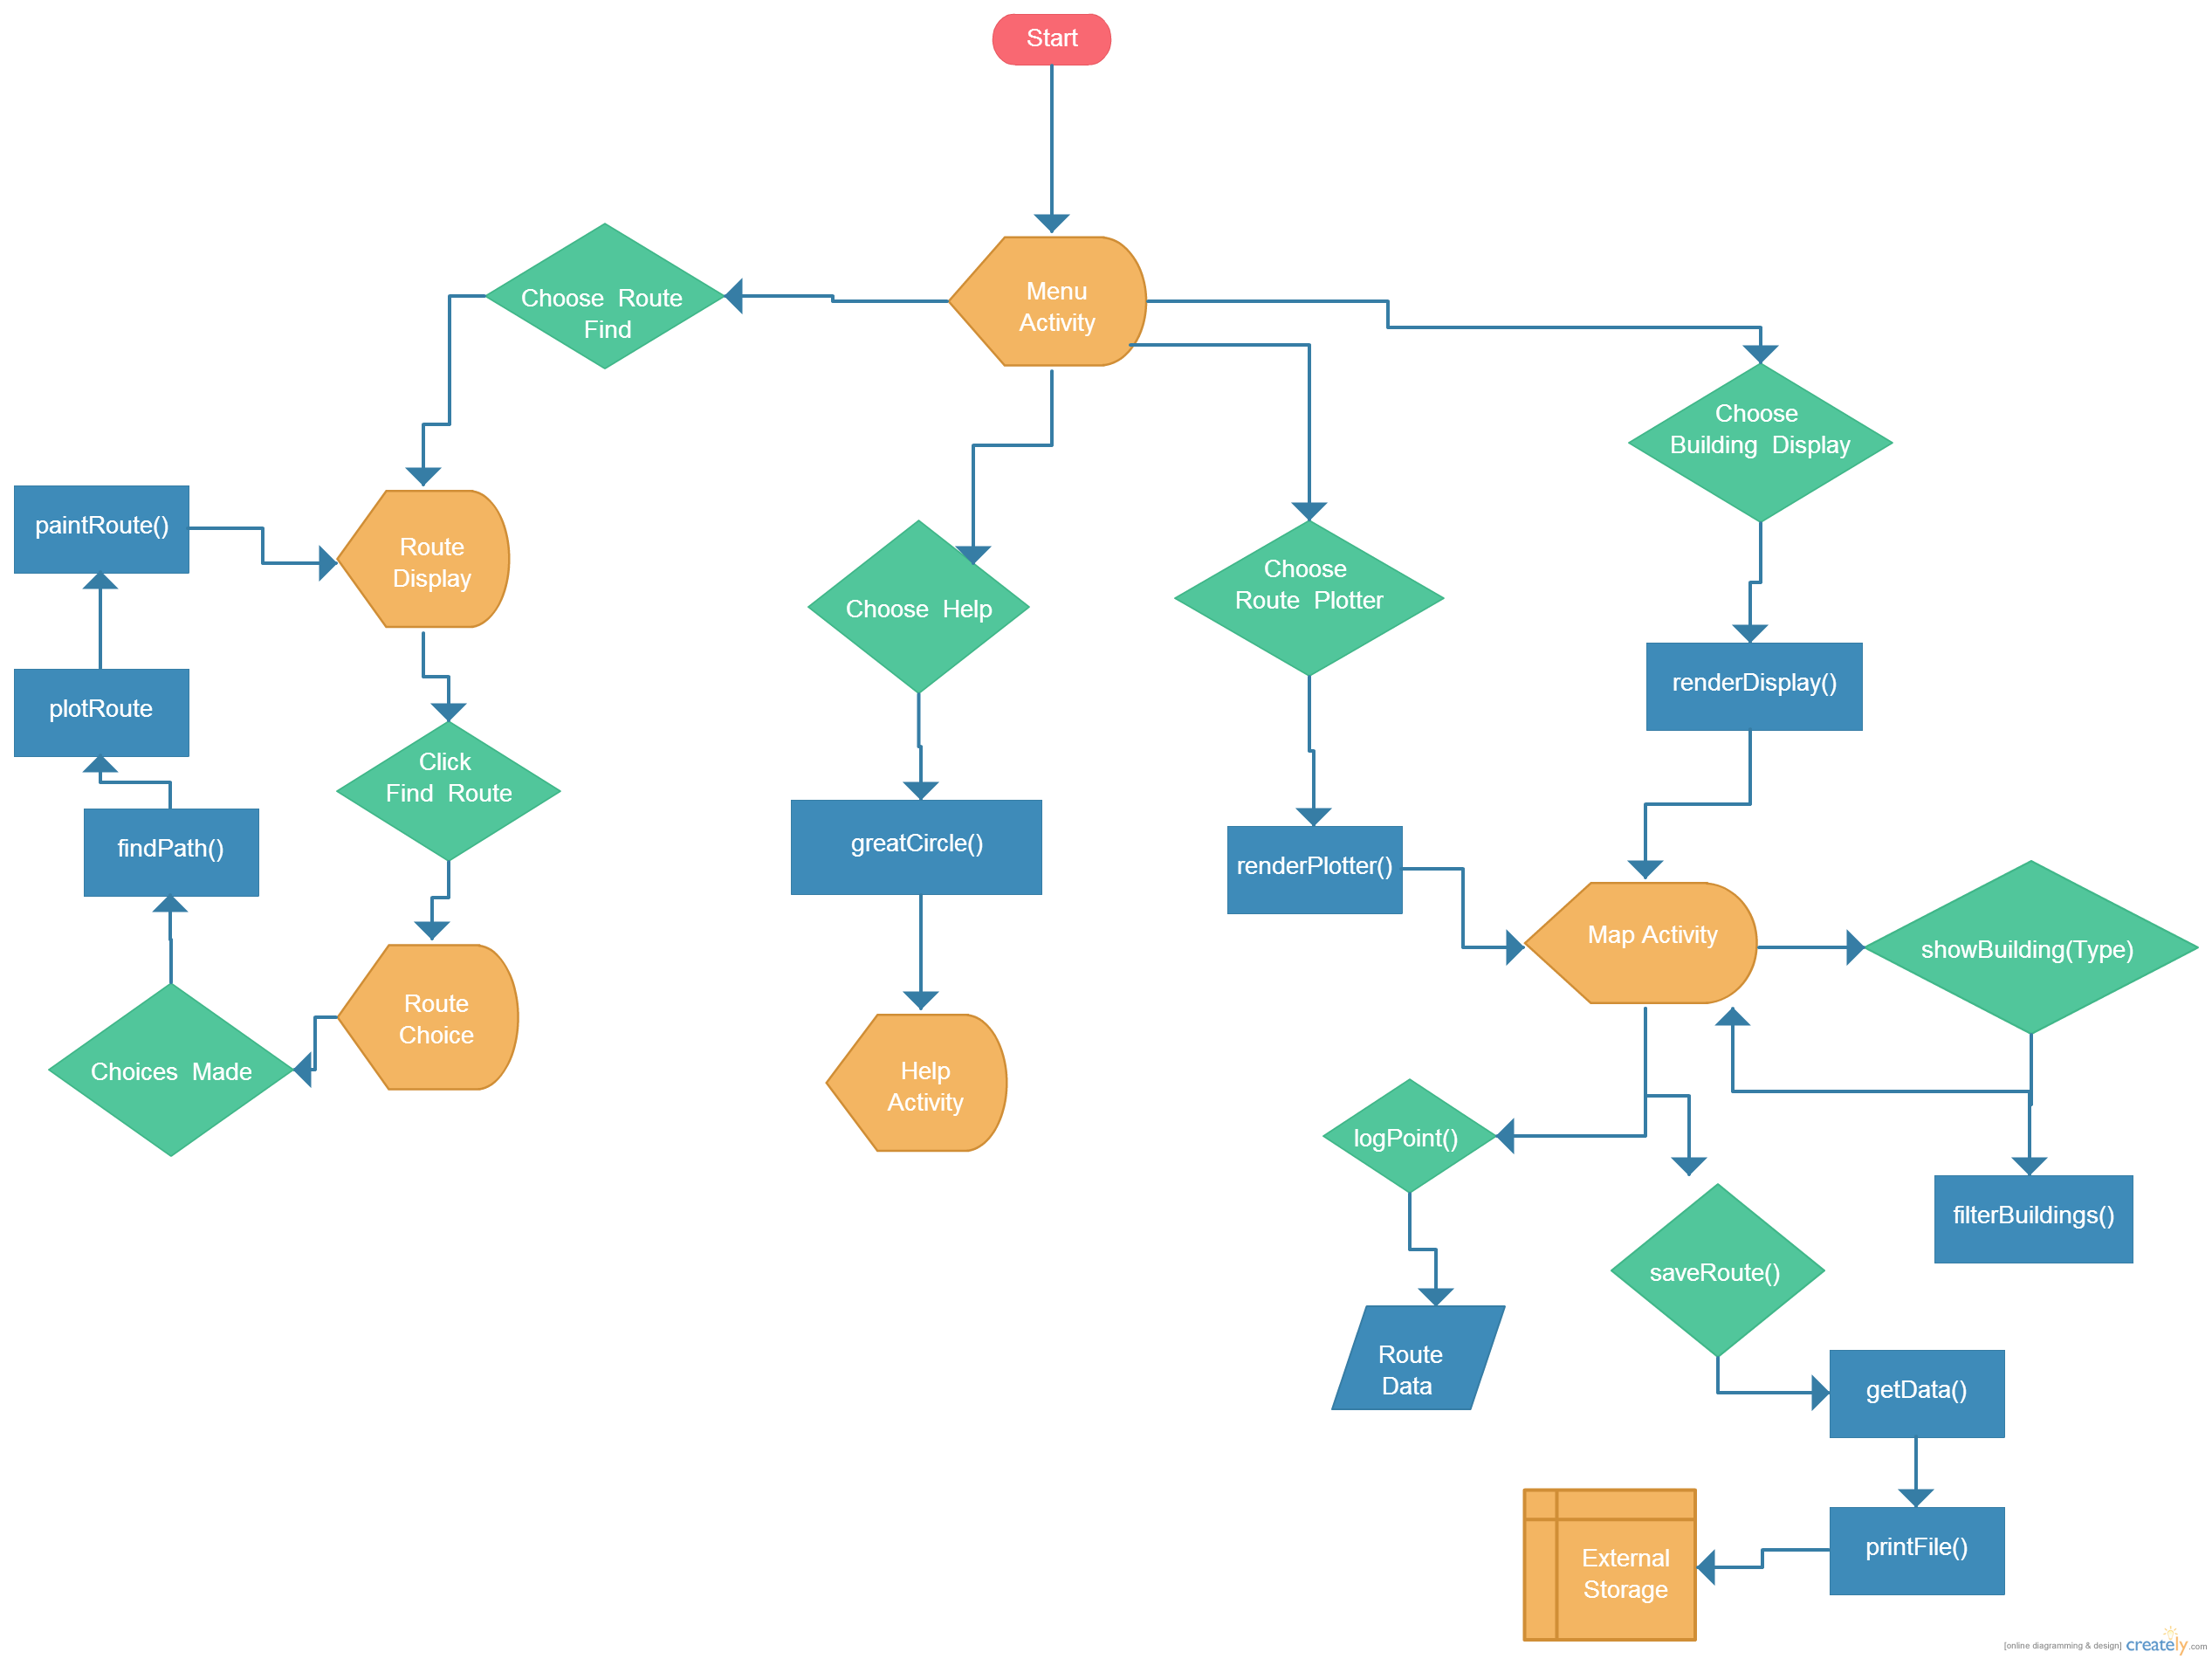
\includegraphics[scale=0.24]{Design/Flow.png}
\caption[Initial Flow Diagram]{Initial Flow Diagram depicting the path a user can follow through the application}
\end{sidewaysfigure}


\newpage
\restoregeometry
\subsection{Class Diagram}
The diagram on the following page describes the estimated architecture of the application, in following is the justification of the current estimated design.
\subsubsection{Justification}
The diagram begins at what is intended to be the root of the application, which branches out into the various activities. The simplest of these activities is the Help Activity, the Help activity has an ArrayList of Place, these represent the locations which will be loaded in through the loadHelpPoints() method. These will then have a distance assigned to them using the calcDist function before finally being sorted by the sortHelpPoints function. The closest will then be displayed using the displayClosest. While split up into several methods here it may be reasonable to merge a couple of them together, this will be decided upon implementation. 

The second activity is the Map activity, which will be rendered based on what the user wants. If the user wants a plotter the user will be able to log a point using logPoint which will be followed by connectPoints, causing a path to appear on the map. Finally the user will want to create a file so createFile will be called causing the creation of the File Printer class which will handle the formatting and output of the data into the correct directory. 

The Map Activity will also be responsible for rendering the view for the viewing of buildings based on filter, filter will be chosen by the user. The buildings will be loaded in using the loadPlaces function which will read the buildings in. A Place also can have a Categories represented by an Enumeration, by doing this it should be easy to put a filter in the showByType function which will then display different Categories based on what the user wants. 

The most complex piece of the diagram is probably the Route Display and its connecting classes. The activity has an ArrayList of Routes which will make up the entire path. This allows us to have different gradings along different parts of our final Paths. The Route Display class will start the Route Choose Activity for a result, in this case the result will be an ArrayList of Routes which will be contained within the returned Intent. 

The Route Choose activity has two expandable list views, which will be populated by the available nodes to travel to in the graph, not all nodes can be travelled to. The options chosen will then be taken and a search performed using the findPath function. The findPath function will return an ArrayList of Routes which will be put into the intent and the Route Display will be returned to.

On return to the Route Display Activity the onActivityResult will be run, which will grant access to the returned Intent object and remove the extras from it using the getRoute method. The path will then be set, which is really setting a possibly long list of smaller Routes. The poly lines used to set the Routes will also be coloured based on their grading. This will be displayed to the user and they will be able to move around the route and have their position displayed using methods native to the Google Maps Android API\cite{maps}. 

This design will be kept to as close as possible during development, due to the design being created in such a way that it provides the modular application we want to finish with. 
\begin{sidewaysfigure}
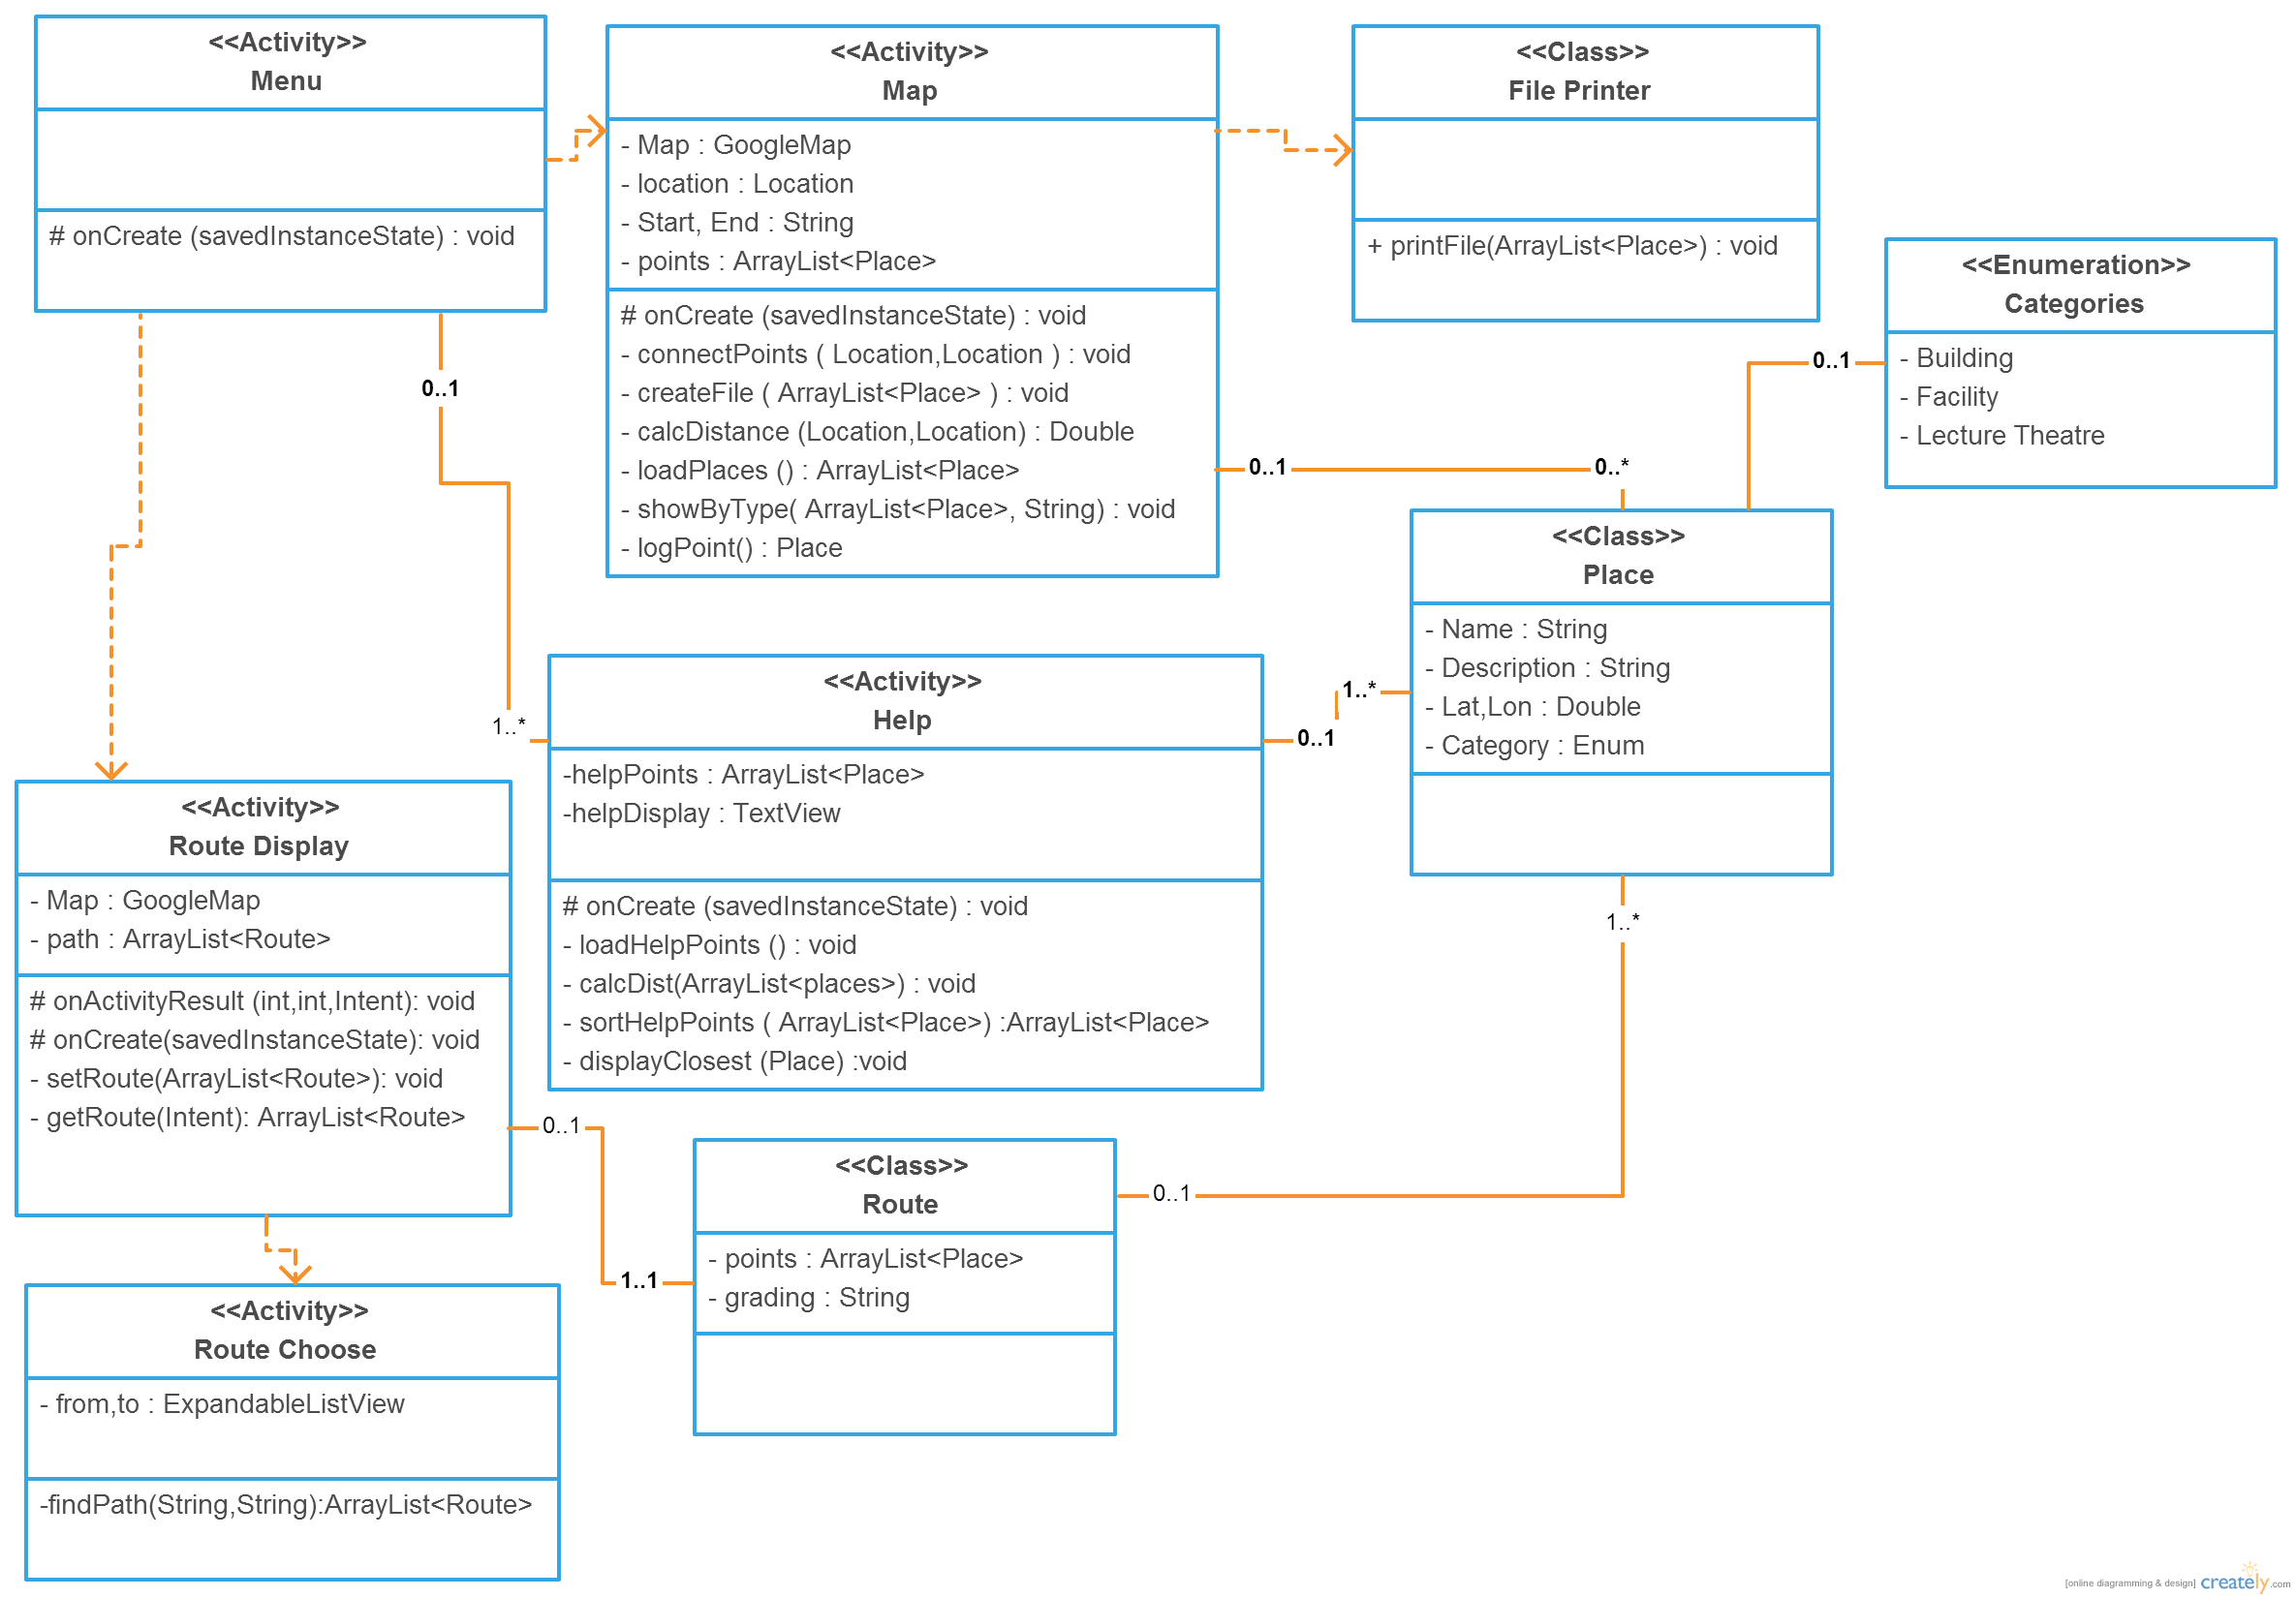
\includegraphics[scale=0.25]{Design/Class.png}
\caption[Initial Class Diagram]{Initial Class Diagram depicting the links between classes in UML notation}
\end{sidewaysfigure}
\newpage
\subsection{Screen Designs}
The following section will include information about the planned Screen Designs and the justification for the proposed designs. Overall the screens have been currently designed to match the colour scheme of the University and as such look as in fitting with the University as it can. It should not be too much problem to have the Screens very closely resemble the designs laid out. 

The button style used throughout the design images shown below will be a custom style written up in XML, various resources can be found on line for both colour picking and XML button design. 
\subsubsection{Menu Screen}
\begin{figure}[h]
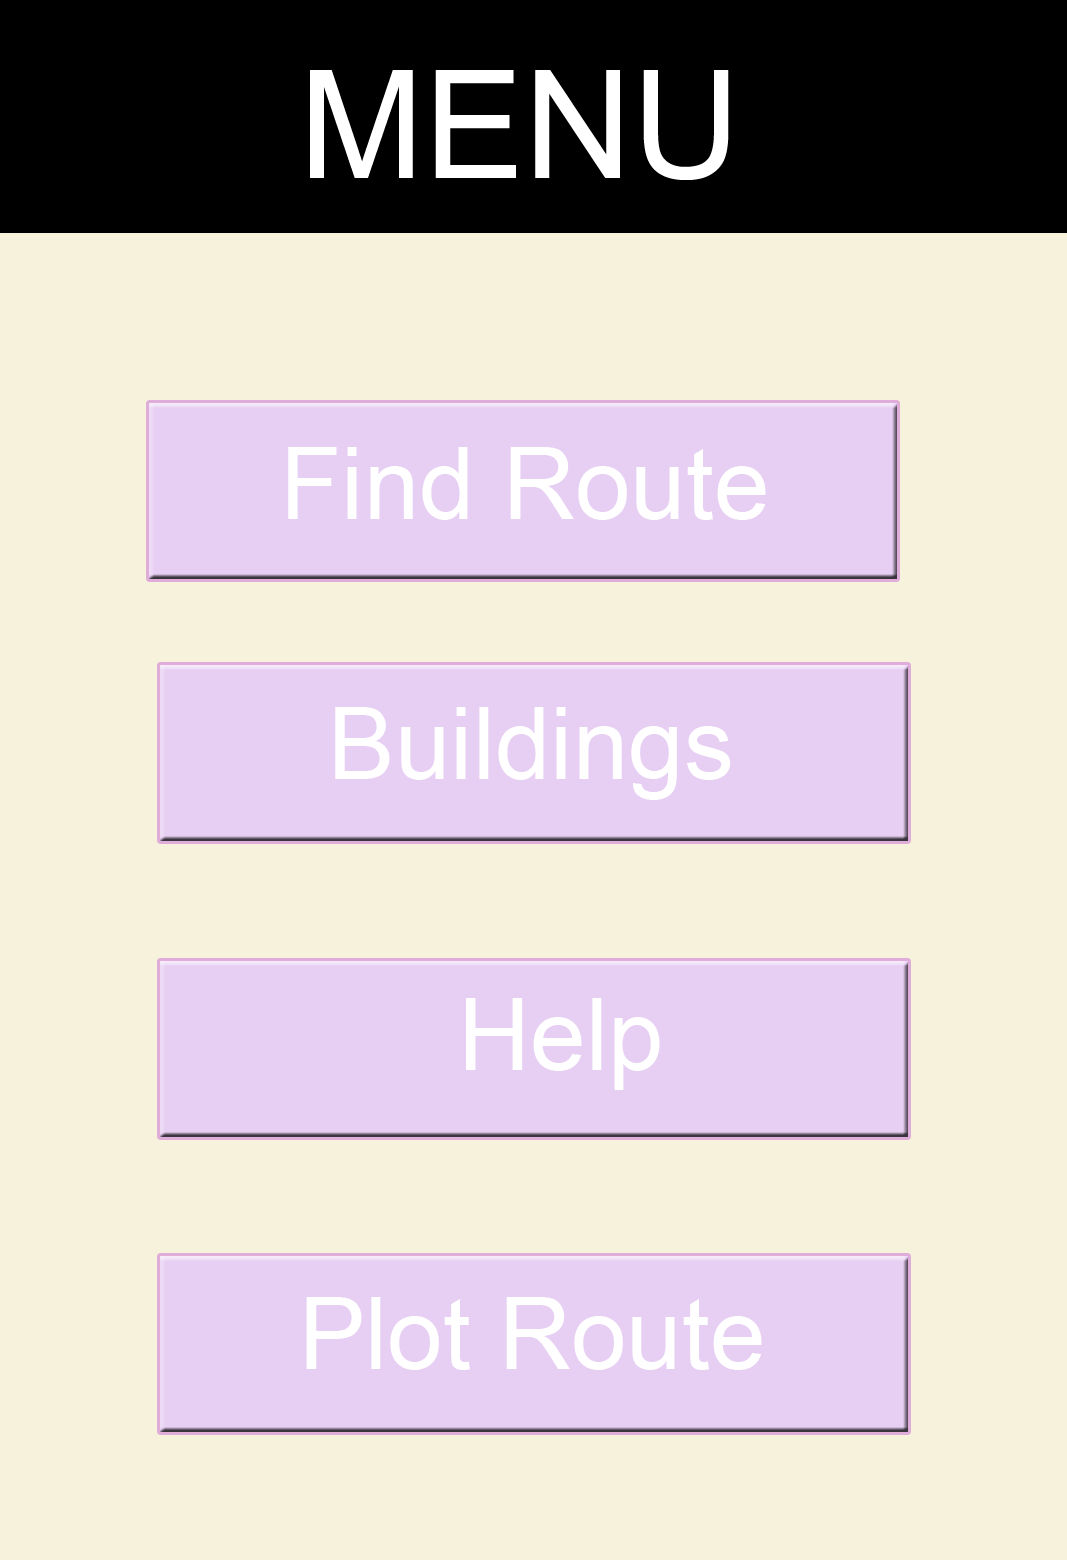
\includegraphics[scale=0.6]{Design/Menu.png}\\
\caption[Initial Menu Design]{Initial Menu Design depicting the predicted layout of the main screen.}
\end{figure}

As can be seen from the above diagram the user will have the label of the current page across the top of the activity, as is common within android applications. The options to move onto the connecting pages will then be arranged within a linear layout and have there respective linked activities as button text. Other options included horizontal buttons but with large screens it could look out of place and be too stretched.

Another possible choice was to have the screens swipe able, so all of the activities are essentially in a row. However after initial research the implementation of this could take long enough to slow down the development of some of the key features. Other possible choices included the inclusion of external libraries, especially some from the 'awesome-android-ui'\cite{aui} package, however it has been decided all design will be developed without the use of outside libraries. If time is available at the end of the projects time line it could be possible to try a test of this for future development. 
\subsubsection{Help Screen}
\begin{figure}[h]
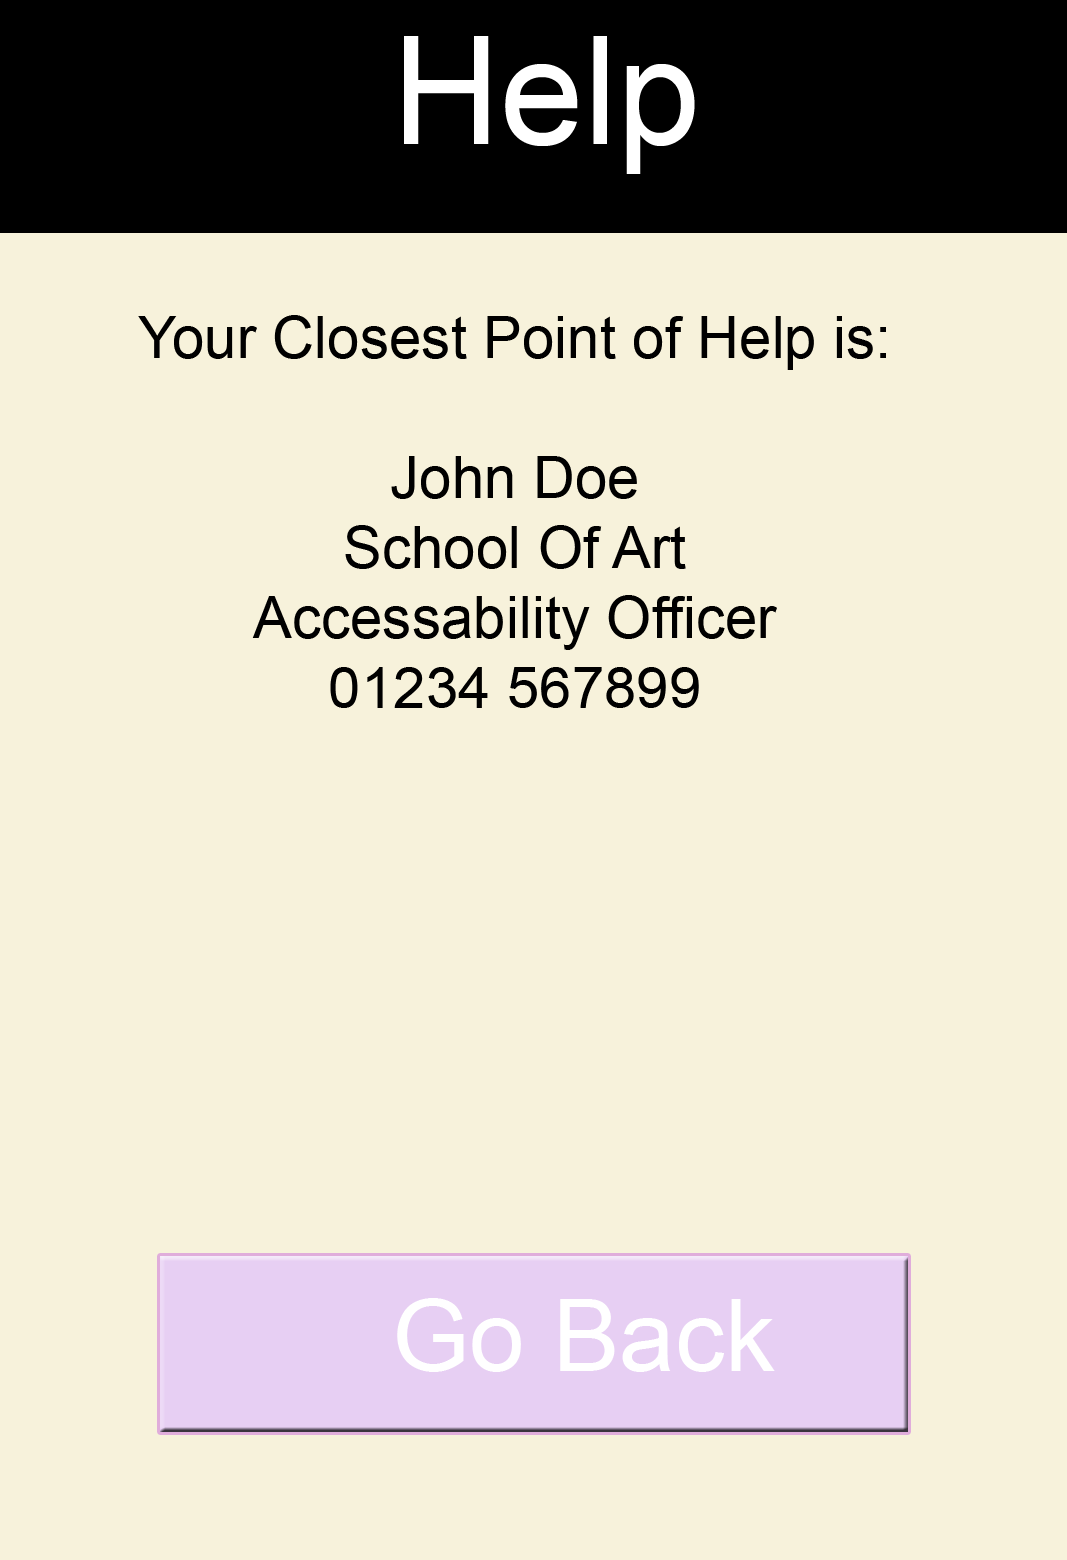
\includegraphics[scale=0.6]{Design/Help.png} \\
\caption[Initial Help Design]{Initial Design for the Help screen, displays information based on user location.}
\end{figure}
The Help screen is again a fairly simple design, the text shown will be a text view which contains the decided location with a button which takes the user back to the Menu Activity. 
\newpage
\subsubsection{Display Buildings}
\begin{figure}[h]
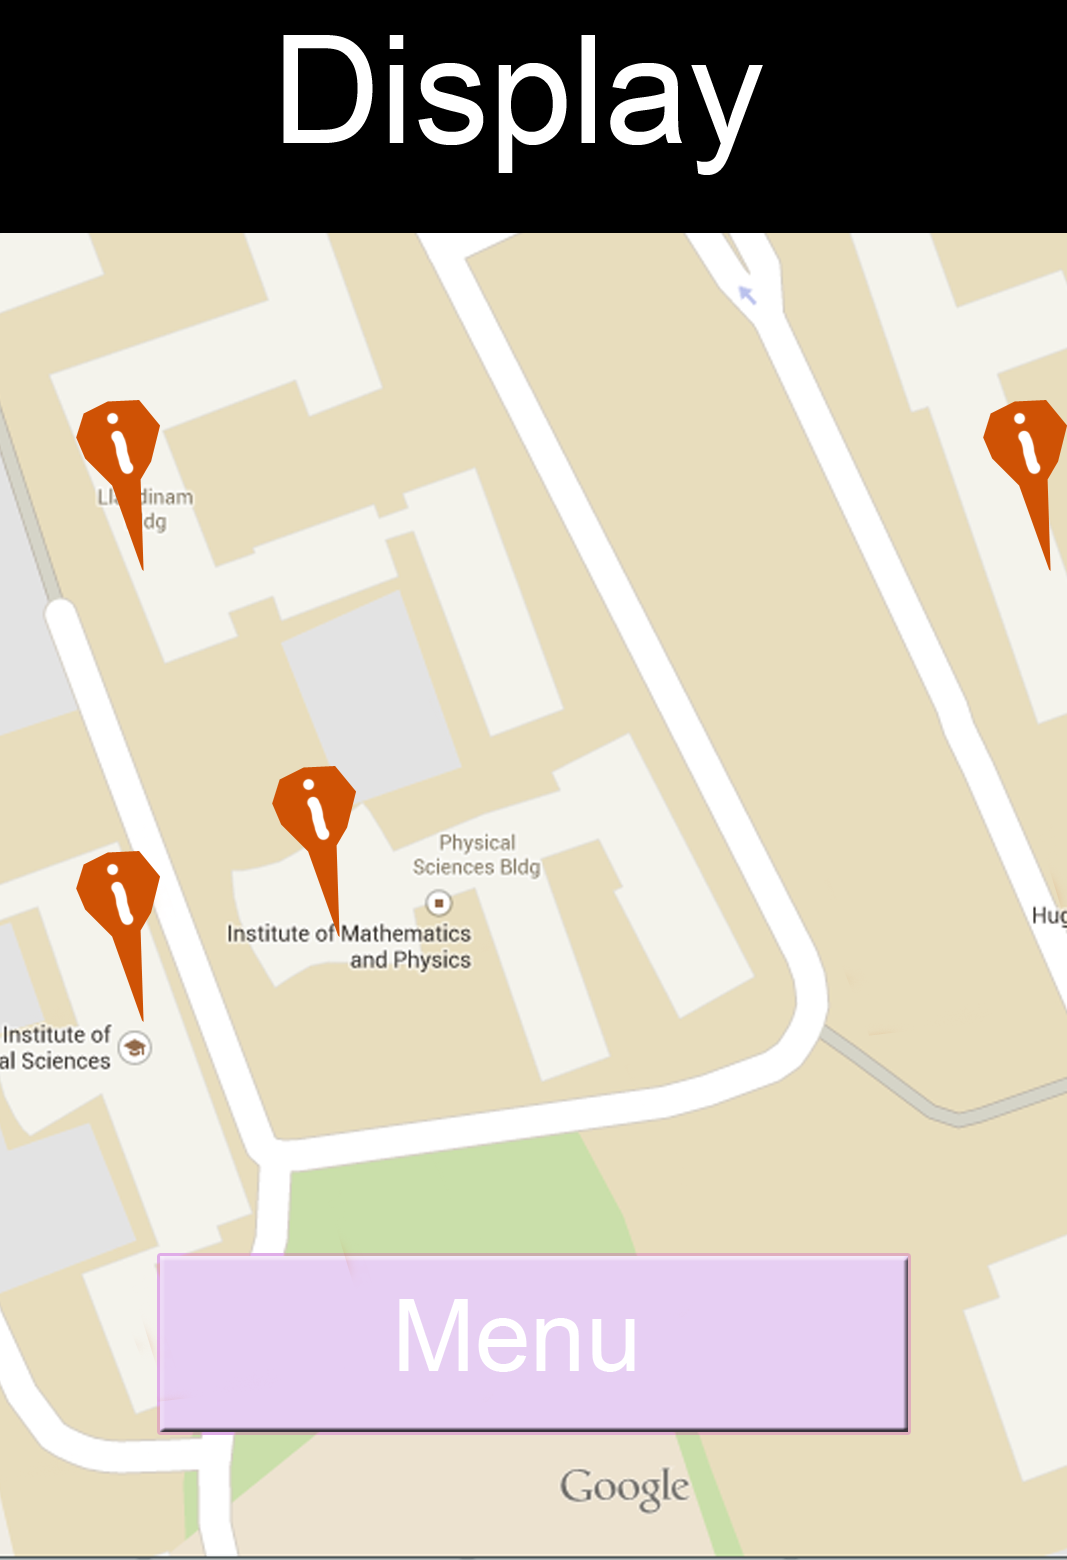
\includegraphics[scale=0.6]{Design/Display.png}\\
\caption[Initial Display Design]{Initial Display Design, view of buildings based on user filtered options.}
\end{figure}
The Display buildings screen will contain a Google Map and have a button which allows for the customisation of which types of buildings are shown. The Menu button will bring up a pop up menu which will allow users to set categories thus showing different markers and there relevant information. 
\newpage
\subsubsection{Route Plotter}
\begin{figure}[h]
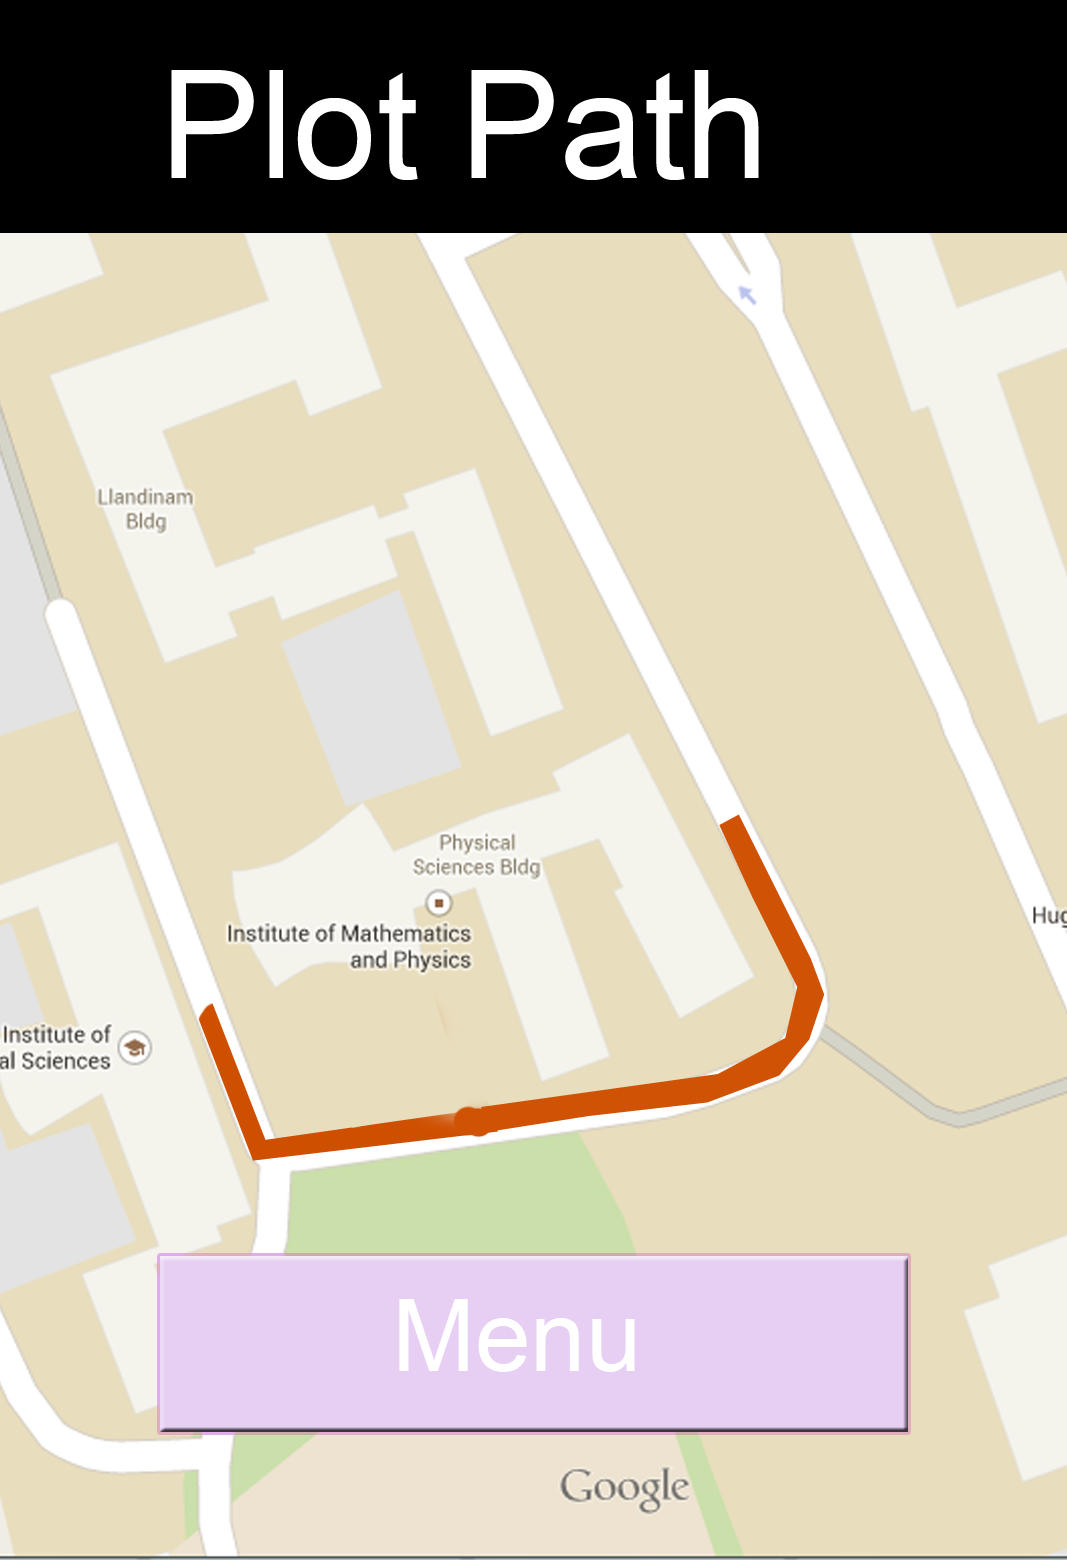
\includegraphics[scale=0.6]{Design/Plot.png}\\
\caption[Initial Plot Design]{Initial design for the route plotting screen for the use of future maintainers.}
\end{figure}
As can be seen from the design the screen will again hold a Menu button, with a pop up menu, which allows the user to choose from a range of options including loggings points, cancelling the current route and saving it to a file. It should also allow for incrementing steps on the route. The Route being walked can be shown on the screen through a use of a set of poly lines.
\newpage
\subsubsection{Route Display}
\begin{figure}[h]
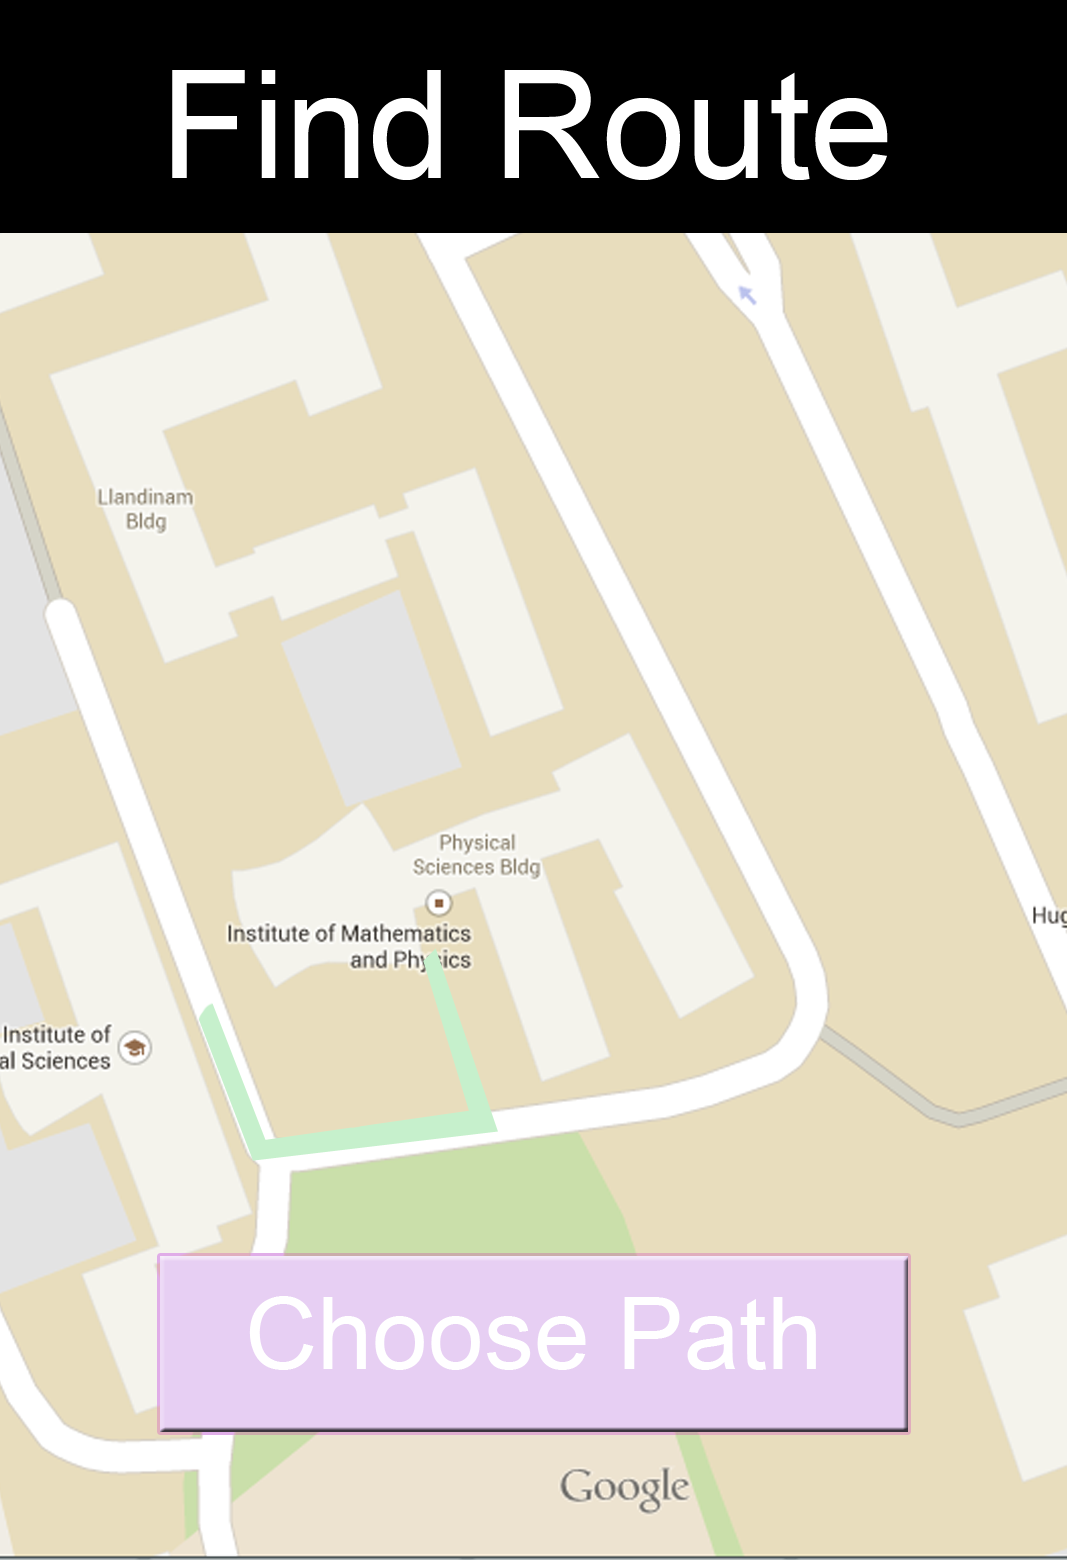
\includegraphics[scale=0.6]{Design/Route.png}\\
\caption[Initial Find Route]{Initial Design for the Route Display Screen including map object.}
\end{figure}
The Route display page the first time it is launched will hold nothing but the map object and a button, as no choice has been made. Afterwards however, as is shown here, the route will be displayed with different colours for segments that range in difficulty.
\newpage
\subsubsection{Route Choice}
\begin{figure}[h]
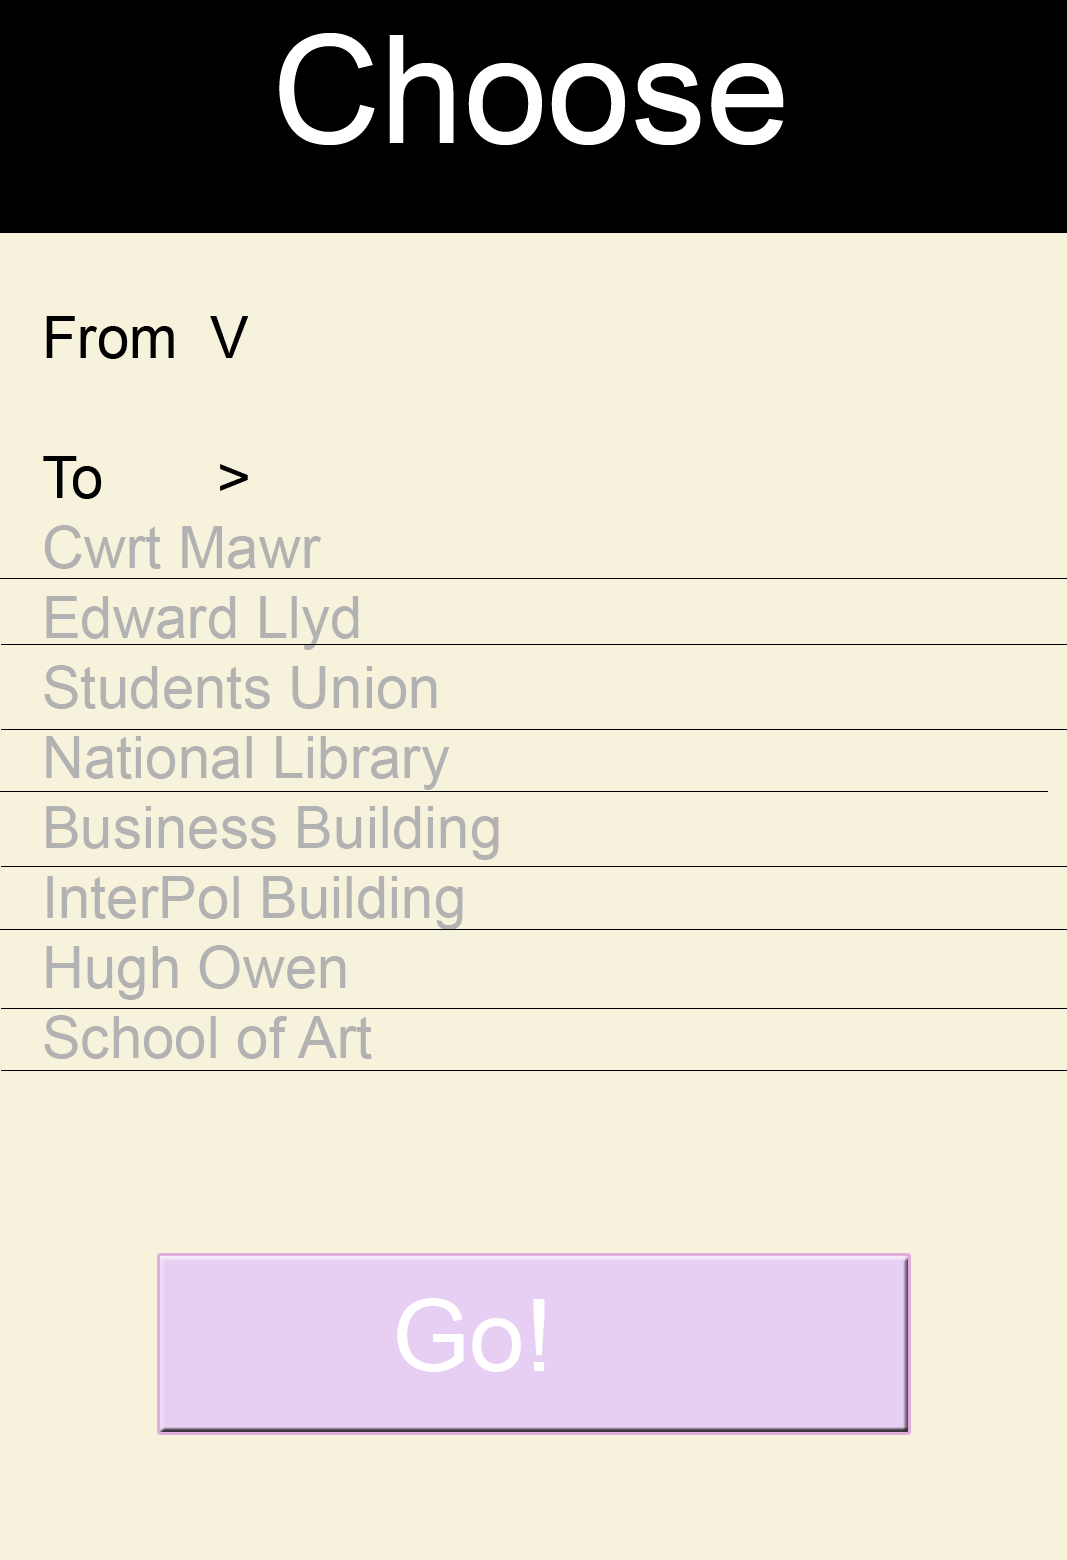
\includegraphics[scale=0.6]{Design/Choose.png}\\
\caption[Initial Route Choice Design]{Initial Screen Design for the Route Choice Activity}
\end{figure}
The final screen that will be included is the route choice screen, containing two expandable list views which will then add the chosen start and destination to the extras for the activity to be passed back. The Button this time will return the user to the Find Route screen which will display the chosen route. 
\subsubsection{Design Notes}
As can be seen the screens try to keep a very consistent style between them, it is felt this is necessary to provide the user with an intuitive experience. Especially in this application due to the criticisms that have been made about the Web version and our access to those criticisms. Other feedback will also be gathered from users meaning that this design could change once that has been gathered. Initial design feedback will be gathered once all screens are functional, it may not be necessary to finish features just their proposed layouts.
